\subsubsection{Mô hình cho tập dữ liệu chỉ bao gồm các quan sát có cột "emailtotal" chỉ là giá trị null}

\begin{enumerate}[label=(\alph*)]
    \item Đầu vào mô hình là vector thu được từ phân tích thành phần chính sử dụng thuật toán PCA
    
    Ta có bảng kết quả huấn luyện mô hình:

    \begin{python}
                        precision    recall  f1-score   support

        Keeping house       0.00      0.00      0.00        55
                Other       0.00      0.00      0.00        23
              Retired       0.38      0.41      0.39       113
               School       0.00      0.00      0.00        13
     Temp not working       0.00      0.00      0.00         8
     Unempl, laid off       0.00      0.00      0.00        19
     Working fulltime       0.49      0.90      0.63       198
     Working parttime       0.00      0.00      0.00        55
     
             accuracy                           0.46       484
            macro avg       0.11      0.16      0.13       484
         weighted avg       0.29      0.46      0.35       484
     
    \end{python}

    và ma trận nhầm lẫn:

    \begin{figure}[H]
        \centering
        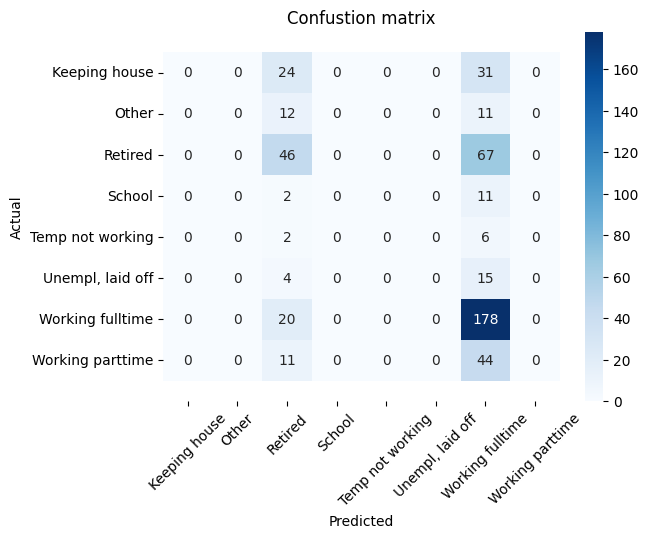
\includegraphics[width=0.6\textwidth]{figures/Thanh/Models/Random_Forest/With_null_models_confusion_matrix_Random_Forest_PCA_features.png}
        \caption{Ma trận nhầm lẫn của mô hình Random Forest khi vector đầu vào được phân tích thành phần chính}
        \label{fig:With_null_models_confusion_matrix_Random_Forest_PCA_features}
    \end{figure}
    
    Ta nhận thấy kết quả phân loại không tốt, trừ nhóm làm việc toàn thời gian có độ hồi tưởng là 0.62 và nhóm đã nghỉ hưu có độ hồi tưởng là 0.41 và độ chính xác là 0.53 thì tất cả độ chính xác và độ hồi tưởng của các lớp khác đều bằng 0.
    Nhìn vào ma trận nhầm lẫn ở hình \ref{fig:With_null_models_confusion_matrix_Random_Forest_PCA_features} ta nhận thấy mô hình dự đoán tất cả các quan sát vào lớp làm việc toàn thời gian.
    Lý do là vì từ phần phân tích dữ liệu, ta thấy phân phối của các thành phần chính tương ứng với các nhóm trong cột wrkstat gần như cùng hình dạng, trộn lẫn vào nhau.
    Mô hình sẽ khó phân biệt được quan sát nào thuộc lớp nào.
    Từ phần dữ liệu, khi vẽ boxplot của thành phần chính tương ứng với các lớp trong cột wrkstat thì cũng có một chút sự khác biệt giữa hai lớp làm việc toàn thời gian và lớp đã nghỉ hưu (\ref{fig:With_null_boxplot_PCA_features_vs_wrkstat_labels}) và hai lớp này có số quan sát lớn nhất.

    Ta sẽ phân tích ngược trở lại trọng số của các tham số tương ứng với các đặc trưng của vector ban đầu từ các tham số ứng với các đặc trưng của các thành phần chính:

    \begin{figure}[H]
        \centering
        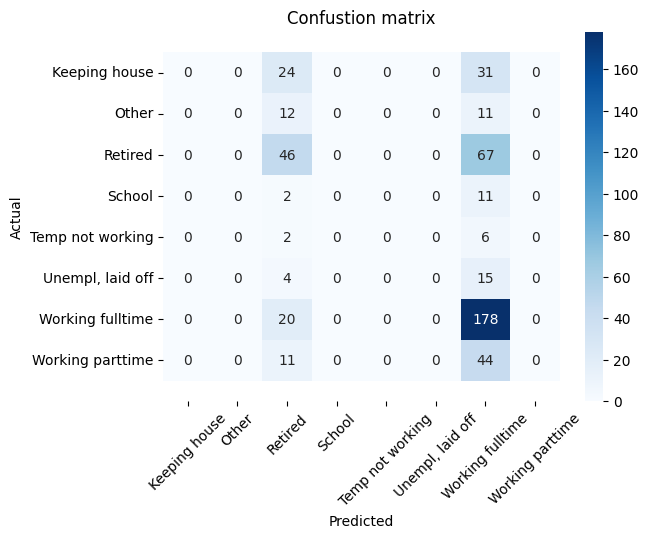
\includegraphics[width=0.6\textwidth]{figures/Thanh/Models/Random_Forest/With_null_models_confusion_matrix_Random_Forest_PCA_features.png}
        \caption{Biểu đồ cột sắp xếp độ lớn giảm dần (trị tuyệt đối) tham số của các đặc trưng}
        \label{fig:With_null_models_confusion_matrix_Random_Forest_PCA_features}
    \end{figure}

    Ta có biểu đồ cột sắp xếp độ lớn giảm dần (trị tuyệt đối) tham số của các đặc trưng thể hiện ở hình \ref{fig:With_null_models_confusion_matrix_Random_Forest_PCA_features}.
    Ta nhận thấy các cột có trọng số lớn và ảnh hưởng nhiều tới các các nhãn đầu ra là harass5\_No và harass5\_Unknown.
    Cả hai đặc trưng trên đều có tần suất xuất hiện lớn trong tập dữ liệu.

    \item Vector đầu vào là vector gốc ban đầu
    
    Ta có bảng kết quả huấn luyện mô hình:

    \begin{python}
                    precision    recall  f1-score   support

   Keeping house       0.00      0.00      0.00        55
           Other       0.00      0.00      0.00        23
         Retired       0.40      0.33      0.36       113
          School       0.00      0.00      0.00        13
Temp not working       0.00      0.00      0.00         8
Unempl, laid off       0.00      0.00      0.00        19
Working fulltime       0.48      0.95      0.64       198
Working parttime       0.00      0.00      0.00        55

        accuracy                           0.47       484
       macro avg       0.11      0.16      0.13       484
    weighted avg       0.29      0.47      0.35       484
    \end{python}

    và ma trận nhầm lẫn:

    \begin{figure}[H]
        \centering
        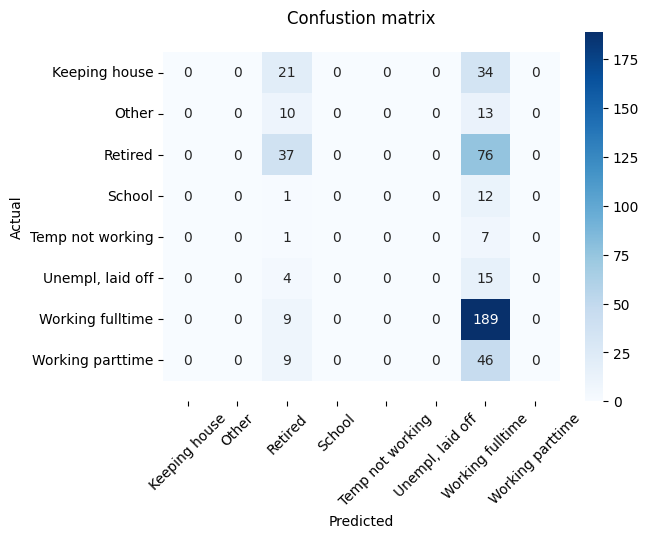
\includegraphics[width=0.6\textwidth]{figures/Thanh/Models/Random_Forest/With_null_models_confusion_matrix_Random_Forest_original_features.png}
        \caption{Ma trận nhầm lẫn của mô hình Random Forest khi vector đầu vào là vector gốc ban đầu}
        \label{fig:With_null_models_confusion_matrix_Random_Forest_original_features}
    \end{figure}
    
    Ta nhận thấy kết quả gần như không khác nhiều so với trường hợp mô hình đầu vào là vector đã được phân tích thành phần chính sử dụng thuật toán PCA.
    Ta nhận thấy có sự đánh đổi về khả năng phân loại đúng của hai nhãn là nhãn làm việc toàn thời gian và nhãn đã nghỉ hưu có sự đánh đổi, thỏa hiệp lẫn nhau.
    Khi kết quả của nhãn làm việc toàn thời gian tăng lên thì kết quả của nhãn đã nghỉ hưu thấp đi và ngược lại.
    Lý do cũng là do từ phần phân tích dữ liệu, ta thấy phân phối của các thành phần chính tương ứng với các nhóm trong cột wrkstat gần như cùng hình dạng, trộn lẫn vào nhau.
    Mô hình sẽ khó phân biệt được quan sát nào thuộc lớp nào.
    Nên rất có thể khi dự đoán một quan sát thuộc vào một lớp nhưng quan sát đó hoàn toàn có thể thuộc về một lớp khác và hai lớp làm việc toàn thời gian và lớp đã nghỉ hưu có số lượng nhiều nhất nên hai lớp này dễ bị phân loại sai giữa lẫn nhau.

    Ta sẽ phân tích ngược trở lại trọng số của các tham số tương ứng với các đặc trưng của vector ban đầu từ các tham số ứng với các đặc trưng:

    \begin{figure}[H]
        \centering
        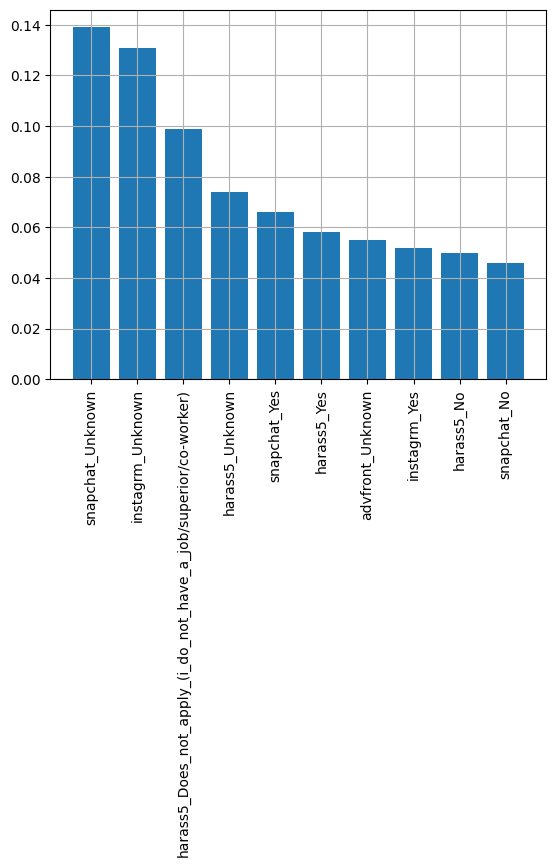
\includegraphics[width=0.6\textwidth]{figures/Thanh/Models/Random_Forest/With_null_models_Feature_Importance_Random_Forest_original_features.png}
        \caption{Biểu đồ cột sắp xếp độ lớn giảm dần (trị tuyệt đối) tham số của các đặc trưng (mô hình với vector đầu vào là vector gốc ban đầu)}
        \label{fig:With_null_models_Feature_Importance_Random_Forest_original_features}
    \end{figure}
    
    Ta có biểu đồ cột sắp xếp độ lớn giảm dần (trị tuyệt đối) tham số của các đặc trưng thể hiện ở hình \ref{fig:With_null_models_Feature_Importance_Random_Forest_original_features}.
    Ta nhận thấy các đặc trưng có trọng số lớn tương ứng với các đặc trưng là snapchat\_Unknown và instagrm\_Unknown đa số là các đặc trưng xuất hiện nhiều trong tập dữ liệu.
\end{enumerate}
